\documentclass{article}
\usepackage[a4paper, total={6in, 8in}]{geometry}
\linespread{1.5}
\usepackage{float}
\usepackage[utf8]{inputenc} 
\usepackage[portuguese]{babel} 
\usepackage{amsmath,amsfonts,amsthm} 
\usepackage{graphicx}
\usepackage{indentfirst}
\usepackage{natbib}
\usepackage{sectsty} 


\newcommand{\horrule}[1]{\rule{\linewidth}{#1}} 
\title{	
\normalfont \normalsize 
\textsc{Escola de Matemética Aplicada} \\
\textsc{Fundação Getulio Vargas}\\ [25pt] 
\horrule{0.5pt} \\[0.4cm] 
\huge Relatório \\ 
\horrule{2pt} \\[0.5cm] 
}


\author{Fernanda Luísa Silva Gomes \\ Gianlucca Devigili \\ João Lucas Duim\\ Juliana Carvalho Souza \\ Raphael Felberg Levy\\[0.1cm]{Professor: Rafael de Pinho André}}
\date{8 de dezembro de 2020} 


\begin{document}
\maketitle

\section{Perguntas de negócio}
O grupo optou por trabalhar com os dados sobre UFC e impacto da COVID-19 no tráfego de aeroportos. Analisando as bases de dados escolhidas, as perguntas foram desenvolvidas com o intuito de realizar amplas análises sobre o material disponível, além de incentivar o uso dos conteúdos aprendidos ao longo das aulas. 
\par As seguintes perguntas foram formuladas em relação à base de dados sobre UFC:
\begin{itemize}
    \item Qual lado ganhou mais?
    \item Quem ganhou mais lutas?
    \item Quantas partidas duraram menos?
    \item Qual peso que tem mais integrantes?
    \item Quem ganhou mais vezes seguidas?
    \item Quem perdeu mais vezes seguidas?
    \item Quantos rounds durou a maior luta?
    \item Qual o máximo de ataques significativos dados pelo lado azul por minuto? 
    \item Quantas derrubadas o lado azul fez a cada 15 minutos?
    \item Quantas vitórias por decisão unânime o lado azul teve? 
    \item Quantos anos tem o lutador mais velho? 
\end{itemize}

\par Em relação à base de dados sobre o impacto do COVID-19 no tráfego do aeroporto, as seguintes perguntas foram formuladas:
\begin{itemize}
    \item Em quais países o número de voos aumentou comparado com o período?
    \item Em que cidades dos EUA o número de voos aumentou?
    \item Em que cidades dos EUA o número de voos diminuiu?
    \item Qual dia teve o maior número de voos internacionalmente?
    \item Qual dia teve o menor número de voos internacionalmente?
    \item Comparando o dia com mais voos com o mesmo dia da semana no período de baselina, o número de voos aumentou ou abaixou?
    \item Comparando o dia com menos voos com o mesmo dia da semana no período de baselina, o número de voos aumentou ou abaixou?
\end{itemize}

\section{Análise dos dados}
\subsection{UFC}
A base de dados fornecida é composta de 4473 linhas e 136 colunas. A base fornece informações sobre o local, vencedor, idade dos lutadores, número de rounds da lutas, entre outros detalhes. Exploraremos os dados, de modo a compreender melhor o perfil dessas lutas. Inicialmente, analisaremos qual lado (vermelho ou azul) ganhou mais.

\begin{figure}[H] 
    \centering 
    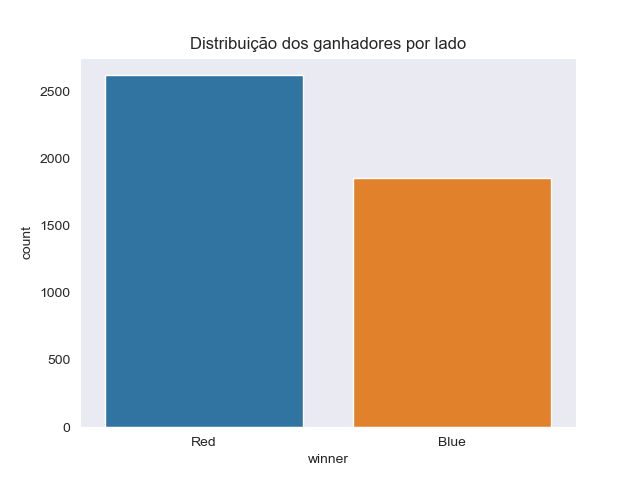
\includegraphics[scale = 0.7]{ganhador_lado.png} 
\end{figure}

\par Apesar de todas as lutas serem dueladas por um lutador vermelho e outro azul e os dois pertencerem a mesma categoria, pela visualização, o lado vermelho ganhou mais lutas com uma diferença considerável.

\end{document}